% Chapter Template

\chapter{Conclusiones y trabajos futuros} % Main chapter title

\label{Chapter4} % Change X to a consecutive number; for referencing this chapter elsewhere, use \ref{ChapterX}

%----------------------------------------------------------------------------------------
%	SECTION 1
%----------------------------------------------------------------------------------------

\section{Conclusiones}

El sistema desarrollado fue instalado en fábrica, con localización en Polonia, cumpliendo satisfactoriamente con su función y logrando una producción de 25000 unidades. Se puede ver el puesto en la Figura \ref{fig:conc1}. Otras imágenes de la fábrica en las Figuras \ref{fig:conc2} y \ref{fig:conc3}.

\begin{figure}[h]
\centering
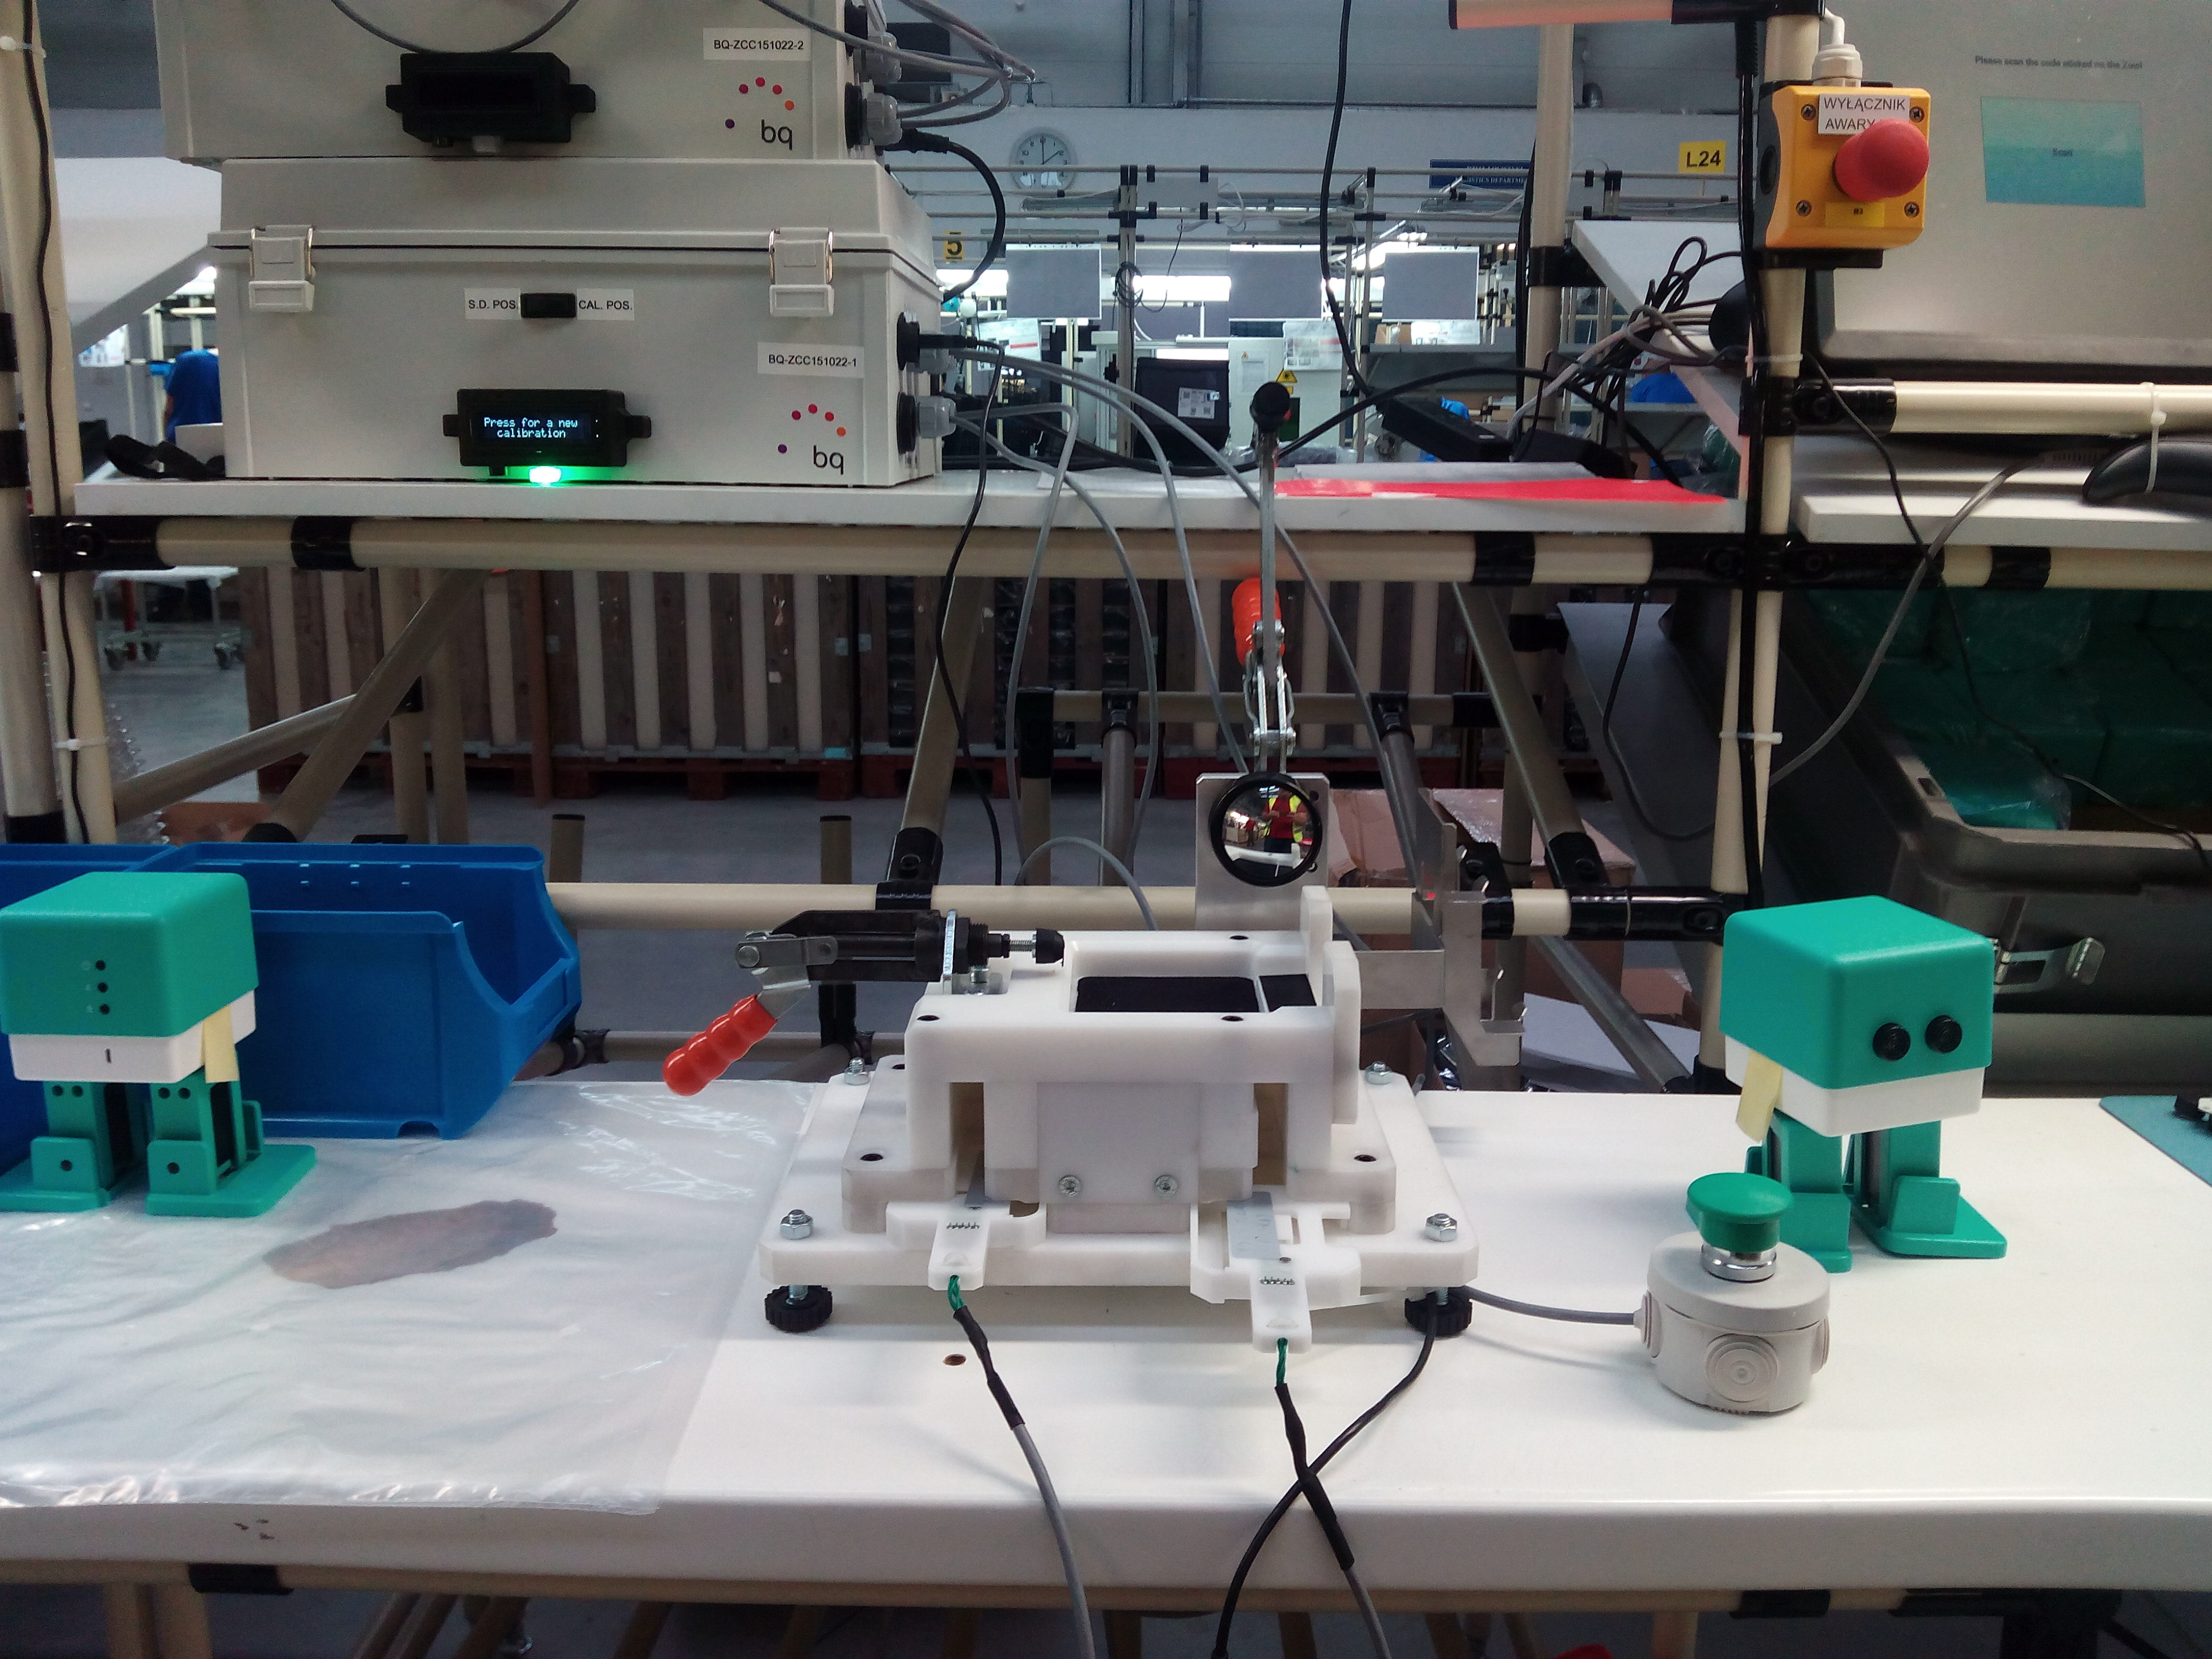
\includegraphics[width=135mm]{Figures/conc1.jpg}
\caption[Puesto de calibración en la línea de montaje]{Puesto de calibración en la línea de montaje}
\label{fig:conc1}
\end{figure}

\begin{figure}
\centering
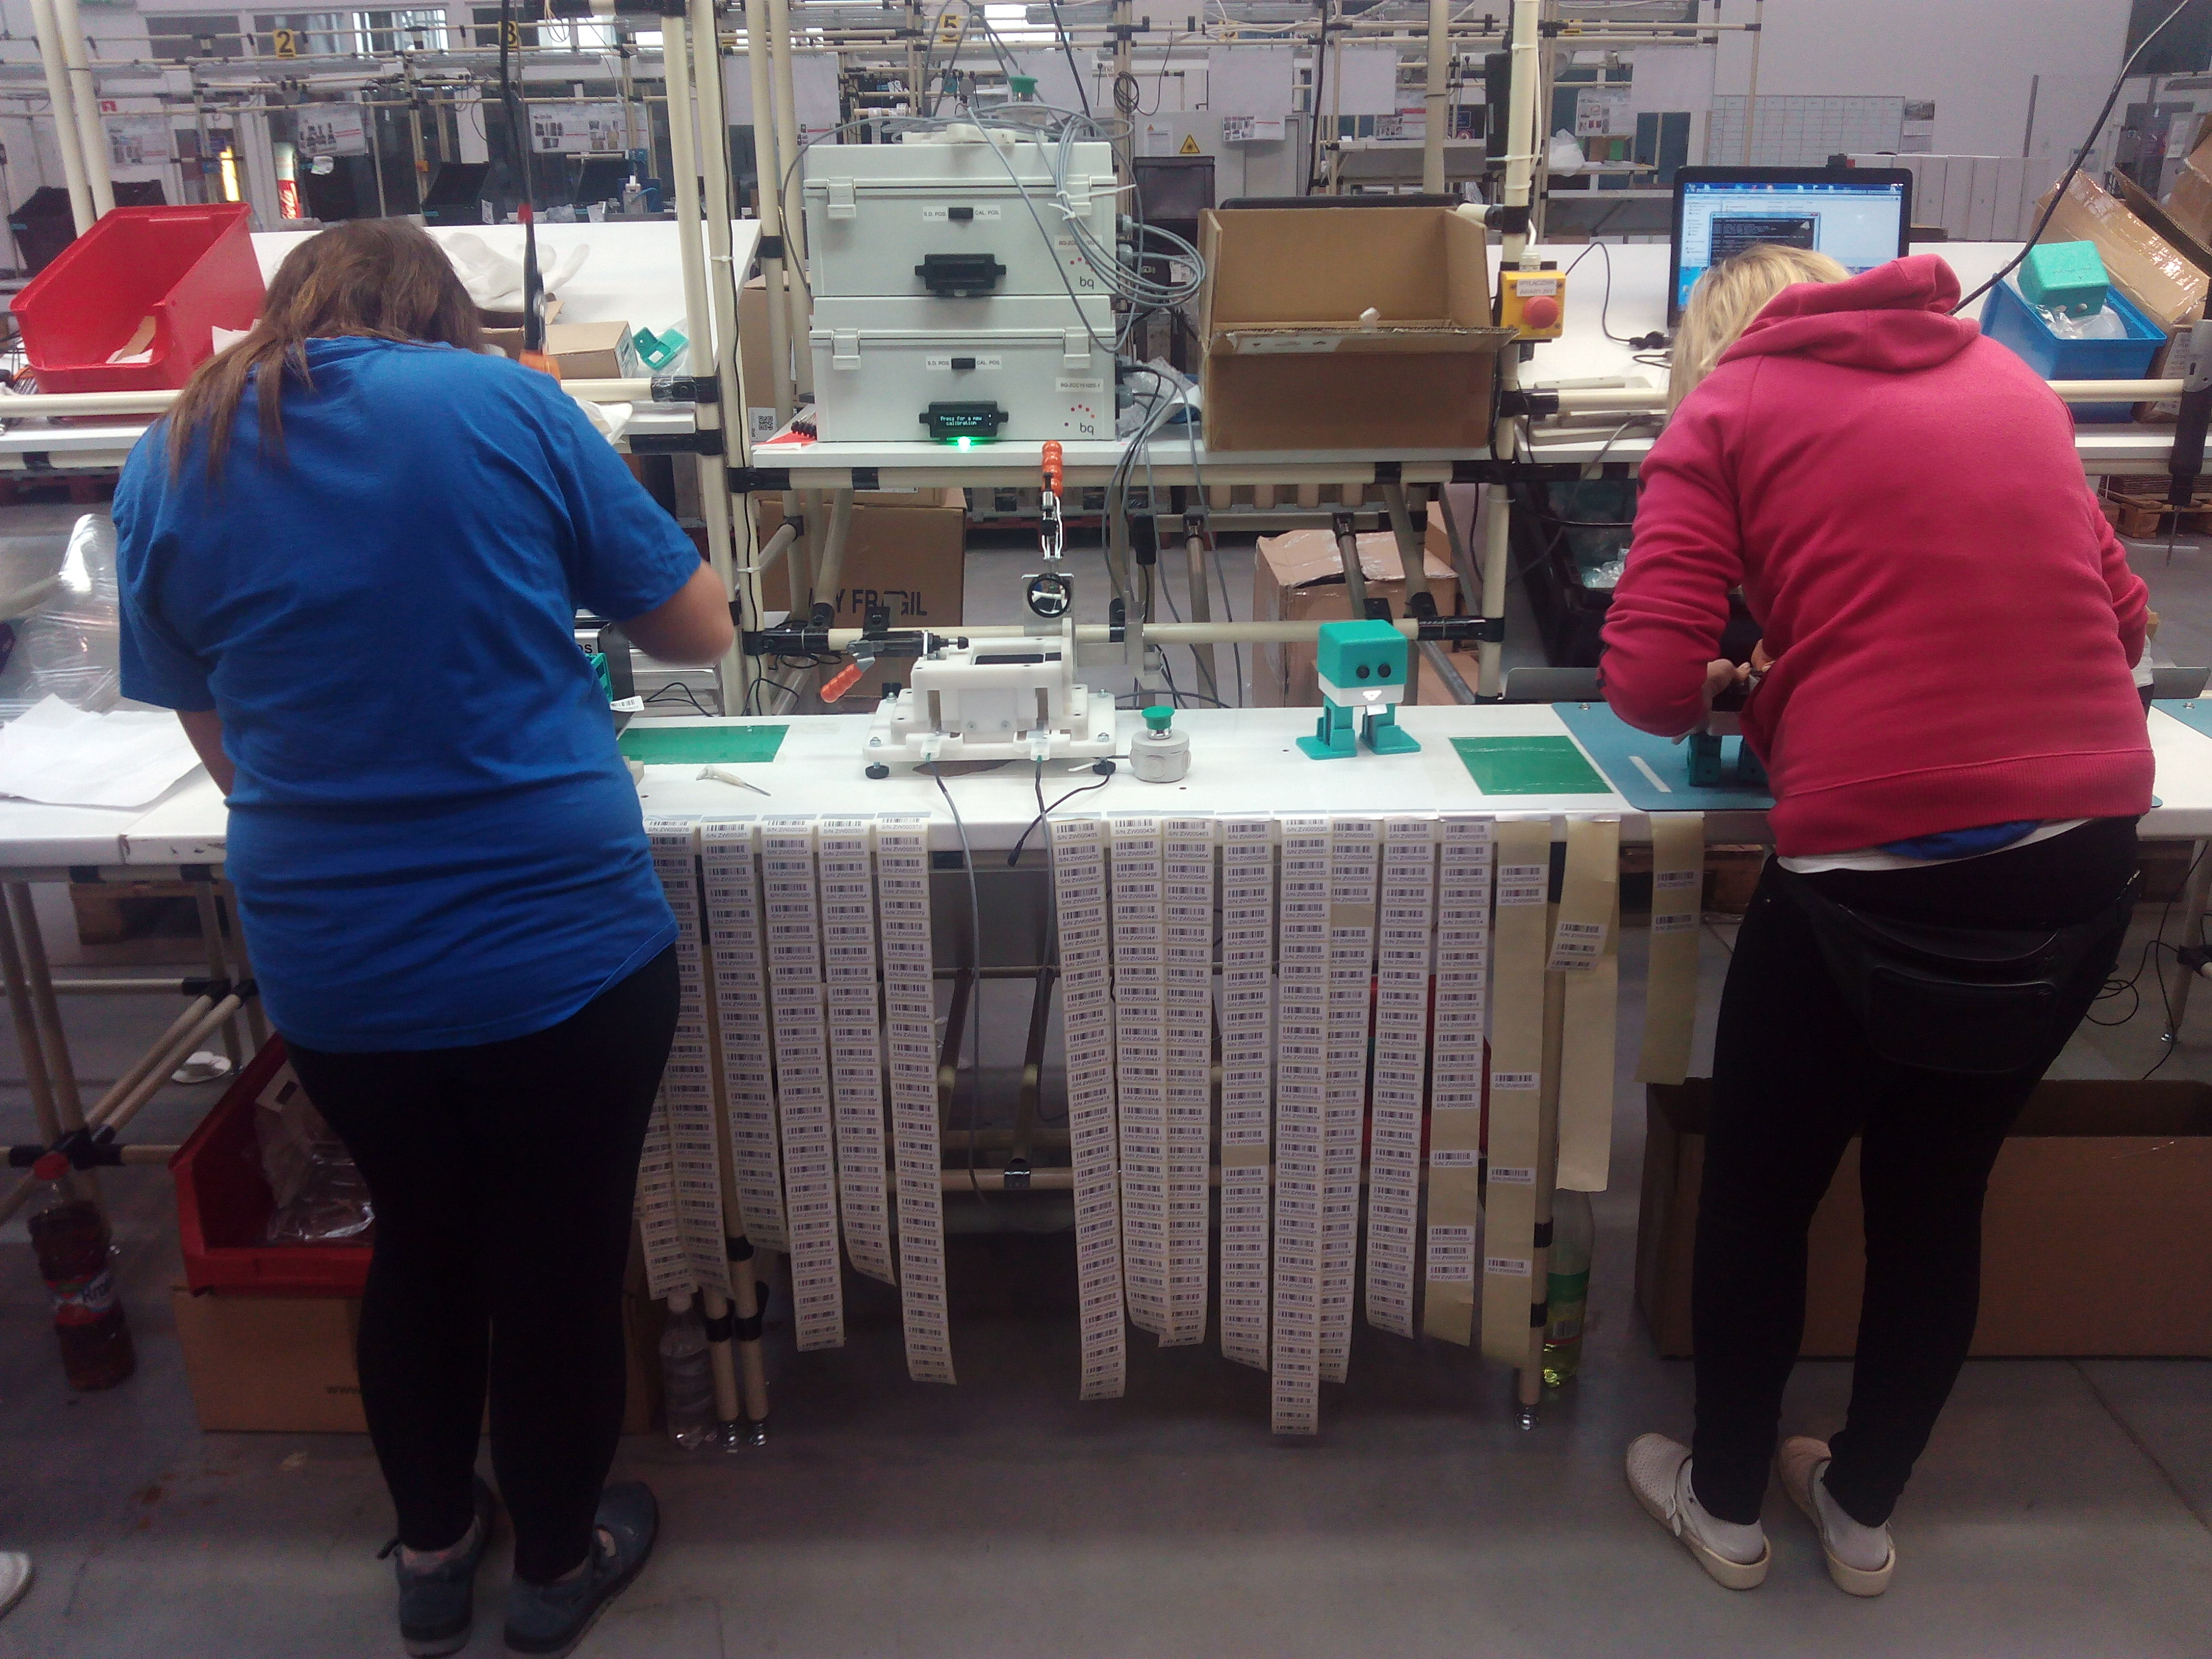
\includegraphics[width=135mm]{Figures/conc2.jpg}
\caption[Operadoras en línea de montaje]{Operadoras en línea de montaje}
\label{fig:conc2}
\end{figure}

\begin{figure}
\centering
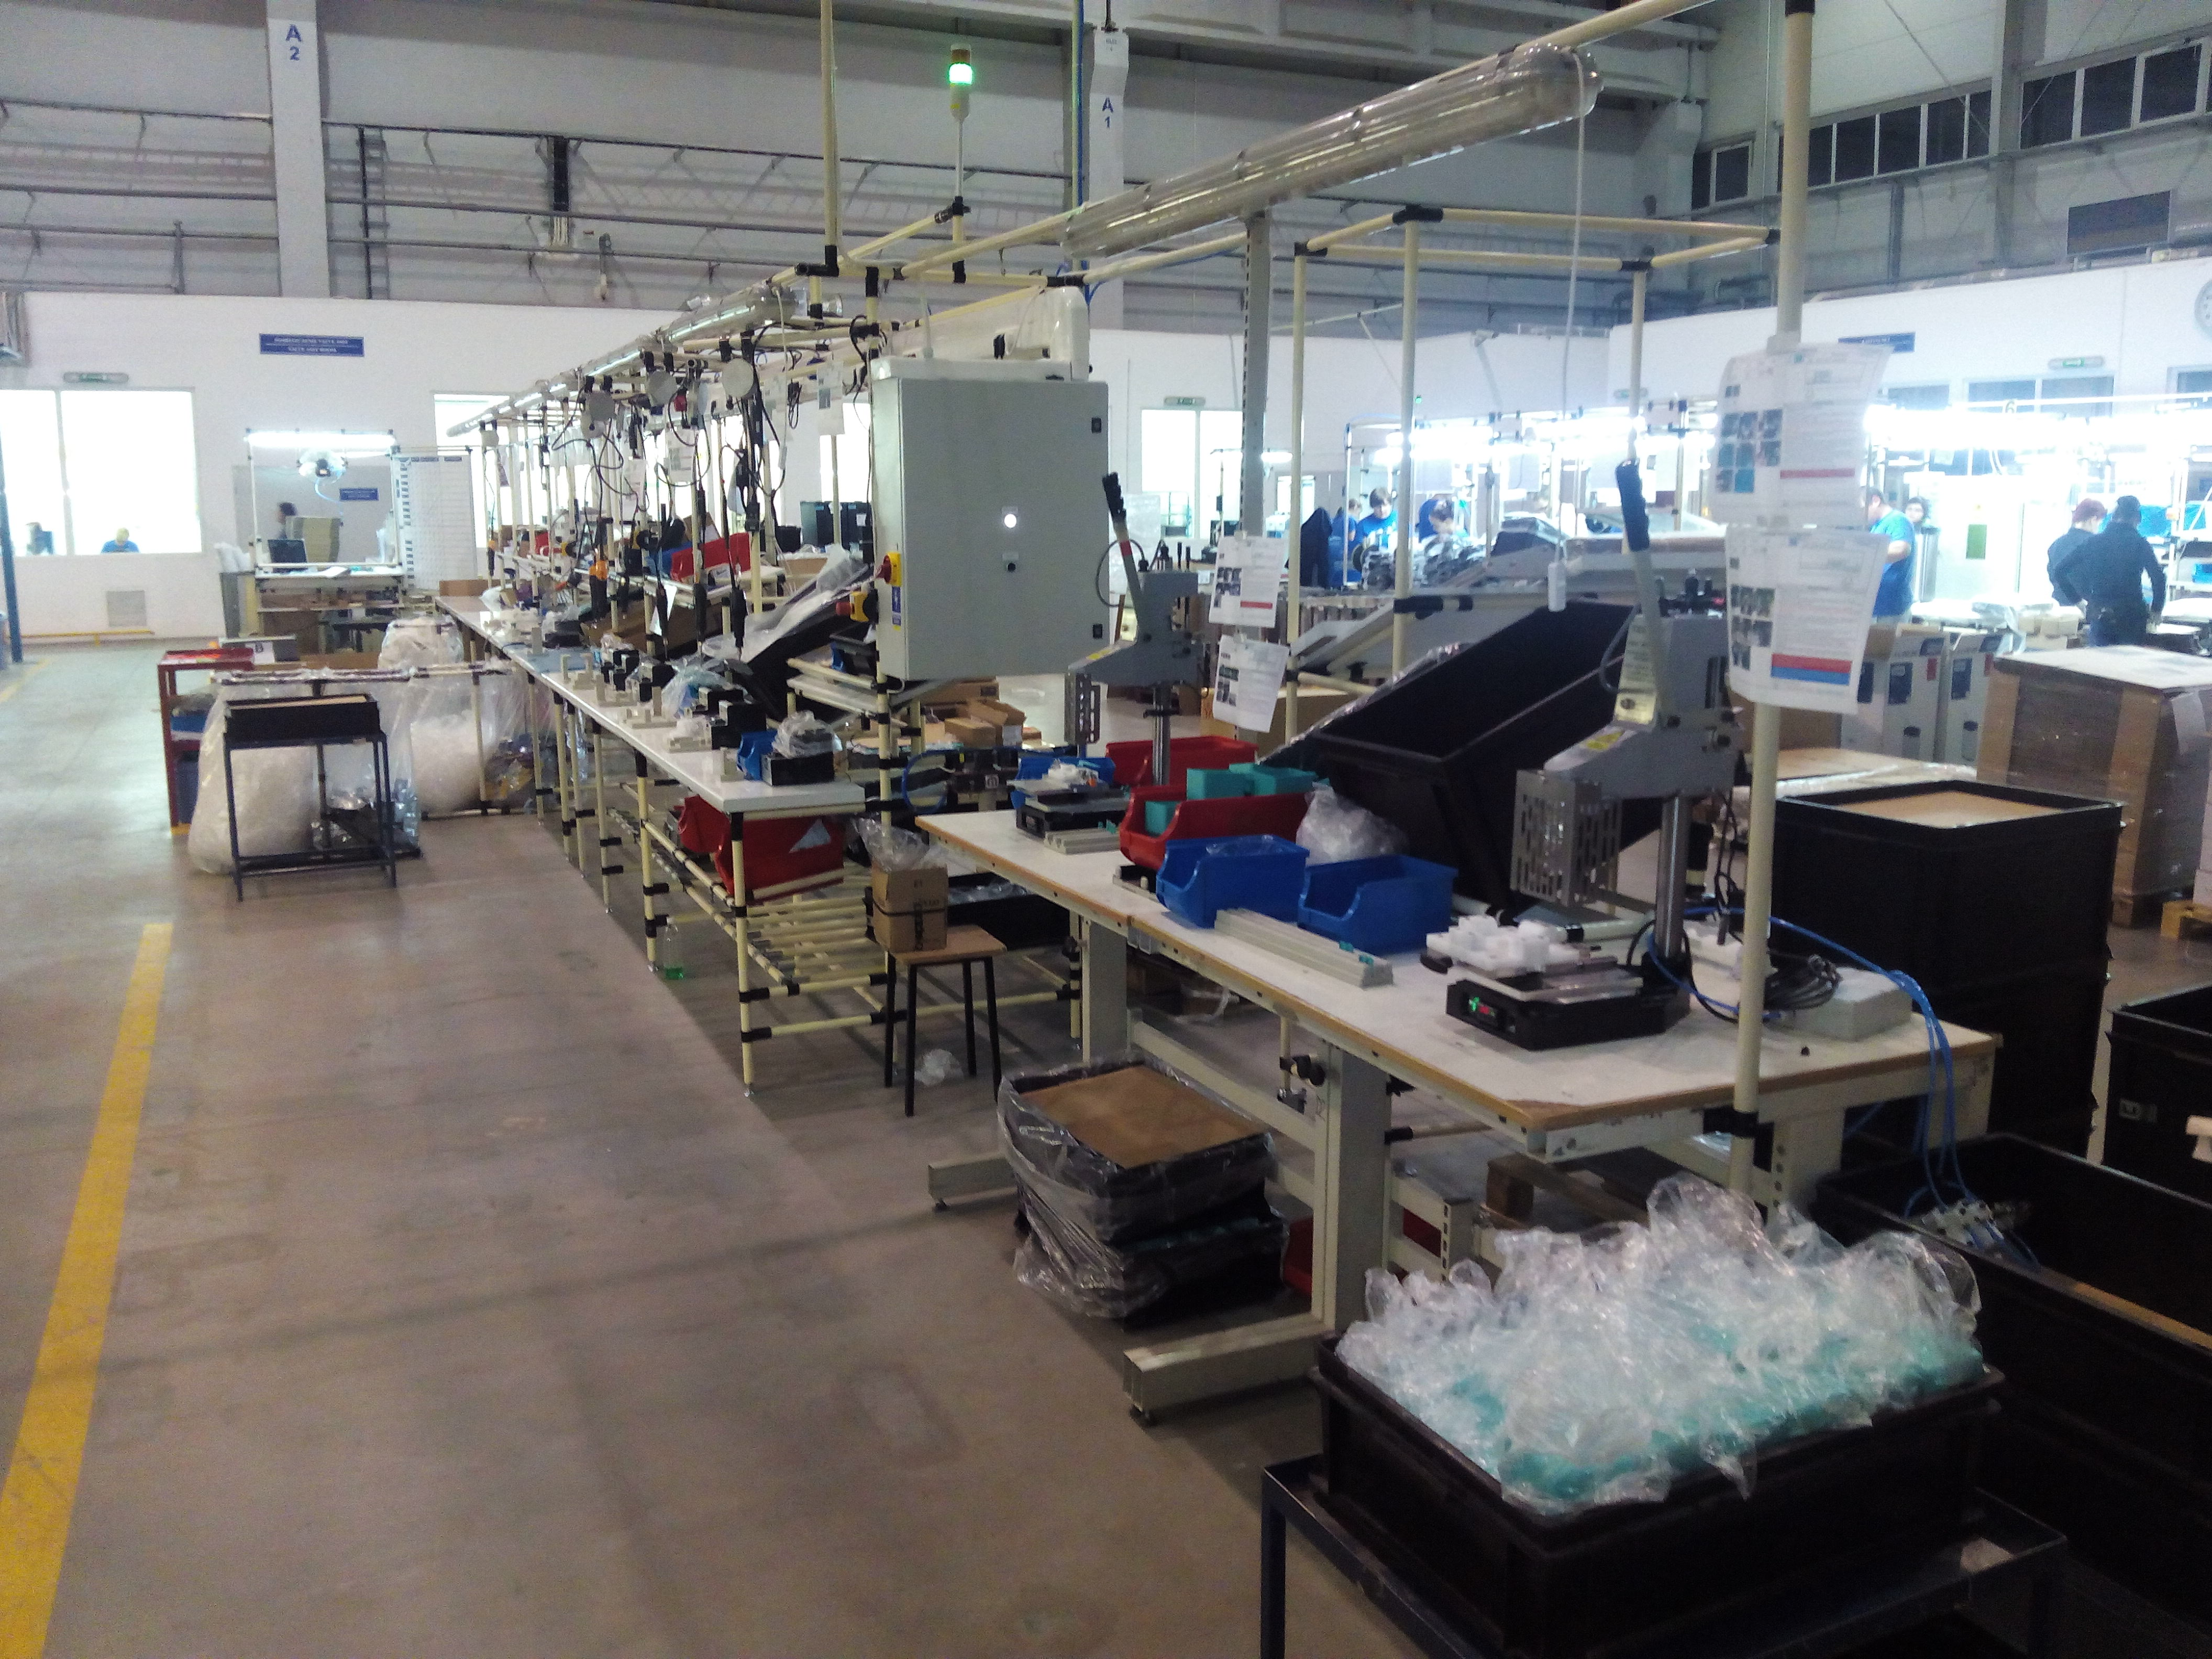
\includegraphics[width=135mm]{Figures/conc3.jpg}
\caption[Línea de montaje de Zowi en Rosti]{Línea de montaje de Zowi en Rosti}
\label{fig:conc3}
\end{figure}

El envío de dos unidades del sistema fue un acierto, en varias ocasiones fue necesario reemplazar componentes o cableado, además de las mejoras implementadas tras los primeros días de operación. Estos contratiempos habrían sido de mayor gravedad si no se contara con el segundo armario.

Los errores más habituales fueron los producidos en el intento de programar la controladora de Zowi: Puerto USB no liberado entre Zowi y Zowi, alta del dispositivo por el SO con otro nombre de puerto, programación de Zowi sin haberlo energizado, desconexión del cable durante la programación... Los dos primeros se solucionaron de forma preventiva, mientras que para los otros dos se aplicaron medidas correctivas.

Los errores podían dejar el sistema totalmente congelado y el reinicio supone una re-calibración de los zapatos, lo que consume alrededor de 2-3 minutos adicionales.

Se observa la base de datos para dos muestras de 4000 unidades -1 semana aproximadamente-. Una muestra al inicio (antes de las mejoras) y otra al final de la producción (tras mejoras). Se atiende a la forma de apagar el sistema: controlado vs. ``botonazo'', confiando en el buen uso de los operadores, como indicador del funcionamiento. Se muestra también el tiempo ciclo entre calibraciones satisfactorias. También el porcentaje de calibraciones ``buenas''. También se muestran ``recuperaciones del sistema'' vs. ``total de veces iniciado''. Estos elementos son indicativos, hay otros factores externos que podrían afectar a los resultados, como un mal montaje de las partes mecánicas del juguete en las etapas anteriores de la línea de montaje, o un mal uso de los operadores, entre otros. Los datos se resumen en la Tabla \ref{tableResults}.

\begin{table}[h]
\centering
\begin{tabular}{l c c}
\toprule
 & \textbf{Pre-mejoras} & \textbf{Post-mejoras} \\
\midrule
Tiempo calibración medio & 81s & 50s \\
Calibraciones a la primera & 98.61\% & 99.13\% \\
Calibraciones OK & 99.76\% & 99.89\% \\
Apagados ``forzados'' & 63\% & 43\% \\
Recuperaciones vs. restarts & - & 35\% \\
\bottomrule\\
\end{tabular}
\caption{Conclusiones y resultados}
\label{tableResults}
\end{table}

\section{Trabajos futuros}

Tras la finalización de la producción inicial, los armarios de calibración y los bancos finales fueron enviados a otra fábrica en Navarra, dónde continúan funcionando.

El último prototipo creado fue actualizado con todos los cambios desarrollados para la versión final. Actualmente se encuentra funcionando en el servicio técnico, utilizando el utillaje diseñado en la fase de desarrollo, Anexo \ref{app:piezas}.

Hablar de futuras mejoras sobre este mismo sistema no tiene sentido ya que el proyecto quedó cerrado y hay otras etapas más lentas en la línea de montaje. Sin embargo, si que se podría haber logrado un mejor diseño, como se comenta a continuación.

Una posible y elegante mejora en la velocidad sería el empleo de un PID en la lectura-actuación de las posición de los servos en lugar del método por iteraciones empleado, o la utilización de sensores y dispositivos electrónicos directamente desde Raspberry.

De cara a otros proyectos utilizando arquitecturas similares (Raspberry y Arduino), donde los plazos y tiempos no jueguen un papel tan importante entre los requisitos, habría algunos puntos a tener en cuenta tras lo aprendido en la realización de este proyecto:

\begin{itemize}
  \item Trabajar en el software: Implementar un logger en las mismas scripts de python y un mayor uso de try-except y comprobaciones que permitan conocer con mayor detalle la traza de operación.
  \item En la misma línea que el punto anterior, utilizar un campo en la estructura de la base de datos para representar qué se está guardando en dicha entrada, esto permitiría identificar fácilmente los diferentes errores, warnings, mensajes informativos...
  \item Desarrollar un pequeño protocolo o herramienta para la comunicación entre Python y Arduino por serie, con una gestión de errores para validación en la interpretación. Dicho protocolo haría más fácil definir en ambos dispositivos las instrucciones que se desean implementar para la comunicación.
  \item El empleo de un reloj RTC (Real time clock) en la Raspberry evitaría la desconfiguración de la hora cuando ésta no tiene acceso a internet y no se puede utilizar NTP para mantener su hora sincronizada.
\end{itemize}
